\chapter{Bridge gros grain}
\label{chap:bridge}

\boitemagique{Objectif}{
L'objectif de ce chapitre est de proposer une fonctionnelle de bridge \textbf{simple} et \textbf{rapide} qui permette de prédire correctement: 
\begin{itemize}
\item Les profils de densité du solvant (g(r))
\item Les énergies libres de solvatation
\end{itemize}
Avec les propriétés thermodynamiques macroscopiques suivantes cohérentes:
\begin{itemize}
\item La bonne tension de surface de l'eau
\item La bonne pression du système
\end{itemize}
}



Comme il à été montré jusqu'ici, l'approximation HNC, y compris corrigée par les bridges décrits dans le chapitre précédent, ne permet pas d'avoir un système thermodynamiquement consistant. 


Nous proposons ici un bridge simple et efficace numériquement, basé sur une densité gros-grain, qui prend en compte le démouillage en permettant la quasi-coexistence des phases gazeuse et liquide de l'eau.
Ce bridge permet donc de retrouver la consistance thermodynamique tout en améliorant les rdfs et les énergies libres de solvatation en échange d'un coût de calcul négligeable.





\section{Le démouillage}
Lorsque de gros composés hydrophobes sont plongés en solution, on observe une transition lente d'une densité quasi-nulle (à la surface du soluté) à la densité bulk (loin du soluté) (voir figure \ref{fig:demouillage}). Ce phénomène est appelé démouillage. Malheureusement, comme on le voit sur la figure \ref{fig:fonctionelle_HNC}, plus on s'éloigne de la densité bulk et plus l'énergie libre d'une unité de volume, soit le potentiel chimique d'une molécule du solvant, augmente. Les phases de faible densité normalement attendues sont donc trop défavorisées pour exister. En réalite, à température ambiante et pression atmosphérique, les phases gazeuses et liquides de l'eau ont la propriété d'être en quasi-coexistence. En effet, comme on le voit sur la figure \ref{fig:diagramme_phase_eau}, à température ambiante et pression atmosphérique, l'eau est proche de la phase gaz. Le potentiel chimique est donc également proche de celui de la phase gaz. Dans l'approximation HNC, les phases de faible densité sont remplacées par des zones de plus forte densité, ce qui entraîne une surestimation forte de la pression du fluide. Comme c'était déjà le cas pour le bridge du 3$^{ème}$ ordre proposé par Jeanmairet et al\cite{jeanmairet_molecular_2013}, nous allons dans un premier temps fixer l'énergie libre de la phase gaz à la même valeur que celle de la phase liquide, soit proche de zéro. Afin d'augmenter la flexibilité du modèle et ainsi de nous permettre d'obtenir une tension de surface correcte, nous ajoutons un nouveau terme d'ordre 4. Afin de calibrer ces nouveaux termes, nous avons effectué une étude paramétrique (décrite plus bas). Le nombre de calcul étant très important, nous avons développé une version spéciale de MDFT adaptée à cette étude: MDFT à symétrie sphérique. 





\begin{center}
    \captionsetup{type=figure}
	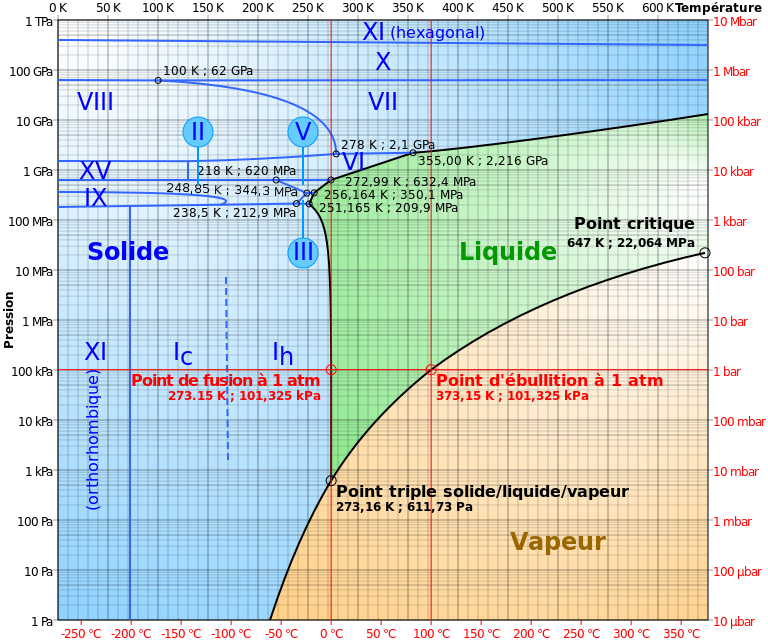
\includegraphics[width=0.8\textwidth]{chapters/bridge/images/diagramme_phase_eau.png}
	\captionof{figure}[Diagramme de phase de l'eau.]{Diagramme de phase de l'eau. Il existe une transition liquid-gaz proche des conditions standards. Cette proximité entraîne la quasi-coexistance des deux phases dans ces conditions. crédit: Olivier Descout}
    \label{fig:diagramme_phase_eau}
\end{center}



\pgfmathdeclarefunction{demouillage}{2}{%
    %\pgfmathparse{1/(#2*sqrt(2*pi))*exp(-((x-#1)^2)/(2*#2^2))}%
    \pgfmathparse{0.5*(tanh(x+#1)+#2)}%
    %0.5*(tanh(x-5)+1)
}

\begin{figure}[ht]
    \center    
  \begin{tikzpicture}
    \begin{axis}[
            xlabel= r (\AA),
            ylabel= densité radiale (kg.L$^{-1}$),
            xmin = 10, xmax = 18,
            ymin = 0, ymax = 2,
            no markers,
            legend style = {draw = none, cells={anchor=west}}
      ]

      \addplot[mark=none, black, very thick, domain=10:20, samples=400] {demouillage(-13.5,1)};
    \end{axis}
  \end{tikzpicture}
    \caption[Représentation du démouillage autour d'une sphère hydrophobe.]{Exemple de densité radiale réaliste autour d'une sphère hydrophobe de rayon R=10 \AA\ en fonction de la distance à la sphère. On attend une densité proche de celle du gaz au contact et la densité bulk de référence de l'eau loin de la sphère.}
    \label{fig:demouillage}
\end{figure}



%\begin{figure}[H]
%  \center
%  \begin{tikzpicture}
%    %liquide
%    \draw[fill=white!70!cyan] (0,0) -- ++(6,0) -- ++(0,6) --++ (-6,0) -- cycle;
%    %gaz
%	\draw[white, fill=white] (0, 0) -- ++(4.5,0) -- ++(-4.5,4.5) -- cycle;
%    \draw[white,fill=white] (4.5,0) arc (0:90:4.5) ;
%    %solute
%    \draw[gray,fill=gray] (0, 0) -- ++(3.5,0) -- ++(-3.5,3.5) -- cycle;
%    \draw[gray, fill=gray, pattern color=black] (3.5,0) arc (0:90:3.5) ;
%    %texte
%    \draw (45:6) node {\large liq};
%    \draw (10:4) node {\large gaz};
%    \draw[white] (45:2) node {\large solute};
%    %contour
%    \draw[black, thick, fill=none] (0,0) -- ++(6,0) -- ++(0,6) --++ (-6,0) -- cycle;
%  \end{tikzpicture}
%    \caption{Démouillage: Un composé hydrophobe plongé dans l'eau va entraîner la création d'une légère couche de solvant gazeuse à son contact.}
%    \label{fig:demouillage}
%\end{figure}



\begin{figure}[ht]
    \center
  \begin{tikzpicture}
    \begin{axis}[
            xlabel= $\rho_{\mathrm{bulk}}/\rho_b$,
            ylabel= $\Delta \mu (\mathrm{kJ.mol}^{-1}.\text{\AA}^{-3}) $,
            xmin = 0, xmax = 1.5,
            ymin = 0, ymax = 0.15,
            scaled y ticks={base 10:2},
            legend style = {draw = none, cells={anchor=west}}
      ]
      \addplot+[mark=none, black, very thick] file {chapters/bridge/datas/fonctionnelles/fonctionnelle.csv};
      \legend{HNC}
    \end{axis}
  \end{tikzpicture}
    \caption[Potentiel chimique d'une molécule de solvant en fonction de sa densité.]{Potentiel chimique d'une molécule de solvant en fonction de la densité $\rho_{\mathrm{bulk}}$ dans l'approximation HNC. $\rho_b$ est la densité bulk de référence de l'eau SPC/E à pression et température standards (1 $\mathrm{kg.L}^{-1}$).}
    \label{fig:fonctionelle_HNC}
\end{figure}





\section{MDFT: version à symétrie sphérique}
Afin de diminuer fortement le temps nécessaire à l'étude paramétrique, nous avons développé une version à symétrie sphérique. Cette version simplifiée repose sur deux approximations:
\begin{itemize}
\item Les solutés étudiés sont neutres
\item Les orientations du solvant sont ignorées
\end{itemize}

La première approximation que nous avons fait est de considérer uniquement des composés neutres.
En effet, les charges permettent la création de liaisons hydrogènes fortes entre l'eau et le soluté ce qui a pour effet de fortement stabiliser ce dernier et ainsi de le rendre hydrophile.
Les composés hydrophobes, entraînant du démouillage sont donc généralement neutres.
Contrairement aux solutés chargés, les solutés neutres forment uniquement des liaisons de Van Der Waals.
Dans le cas du modèle d'eau SPC/E, qui posséde un seul site Lennard-Jones sur l'oxygène, soit en son centre, le soluté n'à aucune inflence directe sur l'orientation des molécules d'eau.
De plus, Jeanmairet et al.\cite{jeanmairet_molecular_2013, jeanmairet_molecular_2016} ont montré que le couplage entre la densité et la polarisation de l'eau est négligeable.
La seconde approximation majeure que nous faisons est donc que chaque orientation du solvant est equiprobable. Cela nous permet ainsi de nous affranchir des angles et de ne considérer qu'une moyenne angulaire de la densité en chaque point de grille.

La symétrie sphérique entraîne une autre différence importante. Au contraire de la version 3D, périodique, les systèmes à symétrie sphériques contiennent par définition un unique soluté dans un solvant infini.

Afin de paramètriser ce nouveau bridge, nous nous concentrons dans une premier temps sur nos molécules modèles: des sphères de Lennard-Jones neutres, avec un solvant sous la forme d'un point et donc sans orientation. L’interaction dépend donc uniquement de la distance entre le soluté et la molécule de solvant. En d'autre termes, tous les points se trouvant sur une sphère centrée sur notre système seront parfaitement identiques. Ces systèmes sont dits à symétrie sphériques. Afin de ne pas minimiser inutilement de nombreuses variables identiques, car équidistantes du centre, nous avons développé une version adaptée de MDFT. Cette version, contrairement à la version 3D, nous autorise à représenter le système sous la forme d'un vecteur 1D de densités partant du centre de notre soluté et allant jusqu'à l'infini et non plus par une grille en 3D. Basé sur ce constat, nous avons adaptée la théorie et nous l'avons implémentée dans une version spécifique de MDFT.



\subsection{La théorie}
Comme nous l'avons décrit précedemment, nous nous affranchissons des orientations du solvant. Cela revient, dans la définition de la fonctionnelle (voir équation \ref{eq:fonctionnelle}) à remplacer $\int\mathrm{d}\Omega\rho(\boldsymbol{r}, \Omega)$ par $\rho(r)$. Dans le cas de coordonnées cartésiennes, le découpage de l'espace se fait sous forme de voxels, alors que dans le cas de coordonnées sphériques, le découpage se fait sous forme de coquilles. L'intégration $\int\mathrm{d}\boldsymbol{r}$ est donc remplacée par $\int\mathrm{dV}_{\mathrm{coquille}}(r)$ avec $\mathrm{dV}_{\mathrm{coquille}}(r)=4 \pi r^2 \mathrm{dr}$, $\mathrm{dr}$ étant l'épaisseur de la coquille soit numériquement, l'espacement entre deux points. Les fonctionnelles idéale et externe, centrées sur l'origine, sont les suivantes:
\begin{eqnarray}
\mathcal{F}_\mathrm{id}(r)&=&\mathrm{k_B}T\int\mathrm{dV}_{\mathrm{coquille}}(r) [ \rho\left(r \right)\ln\left(\frac{\rho\left(r \right)}{\rho_0}\right)-\rho\left(r \right)+\rho_0 ],\\
\mathcal{F}_\mathrm{ext}(r)&=&\int\mathrm{ dV}_{\mathrm{coquille}}(r)\rho\left(r \right)\phi\left(r \right)\\
\end{eqnarray}
Au contraire des deux premiers termes, la fonctionnelle d'excès n'est pas centrée sur l'origine. Nous ne pouvons donc pas nous placer directement dans des coordonnées sphériques. Nous réécrivons donc dans un premier temps cette partie de la fonctionnelle sous la forme d'une convolution, ce qui nous donne :
\begin{eqnarray}
\mathcal{F}_\mathrm{exc}(r) &=& \mathcal{F}_\mathrm{hnc} + \mathcal{F}_\mathrm{b}
\end{eqnarray}
Avec
\begin{eqnarray}
\mathcal{F}_\mathrm{hnc}&=& -\frac{\mathrm{k_B}T}{2}\int\mathrm{d}\boldsymbol{r} \Delta\rho\left(\boldsymbol{r} \right)  \int\mathrm{d}\boldsymbol{r}^\prime c_s\left(\left|\boldsymbol{r}-\boldsymbol{r}^\prime\right| \right) \Delta\rho\left(\boldsymbol{r}^\prime \right) + \mathcal{F}_\mathrm{b}\\
						 &=& -\frac{\mathrm{k_B}T}{2}\int\mathrm{d}\boldsymbol{r} [ \Delta\rho\left(\boldsymbol{r} \right)  *\gamma(\boldsymbol{r}) ] + \mathcal{F}_\mathrm{b}
\end{eqnarray}
 avec $\gamma(\boldsymbol{r}) = \int\mathrm{d}\boldsymbol{r}\mathrm{d}\boldsymbol{r}^\prime c_s\left(\left|\boldsymbol{r}-\boldsymbol{r}^\prime\right| \right) \Delta\rho\left(\boldsymbol{r}^\prime  \right)$ et $c_s$ la contribution à symétrie sphérique de la fonction de corrélation directe totale. À condition d'utiliser une convolution adaptée, nous sommes ici autorisés à réécrire cette partie de la fonctionnelle dans les coordonnées sphériques. Nous obtenons ainsi:
\begin{eqnarray}
\mathcal{F}_\mathrm{hnc} &=& -\frac{\mathrm{k_B}T}{2} \int \mathrm{d} r (\Delta\rho\left(r \right)  \ast (\gamma(r)) + \mathcal{F}_\mathrm{b}
\end{eqnarray}
Une résolution rapide et simple de ce terme est décrite plus loin.




\subsection{Implémentation}
Une version de cette théorie à été implémentée dans un code de 2800 lignes de C++ objet haute performance. Comme nous l'avons décrit ci-dessus, l'espace est représenté par un ensemble régulier de densité allant du centre du système jusqu'à l'infini. Numériquement, nous avons limité le vecteur à un ensemble de densités réparties entre l'origine et une distance suffisamment loin pour ne plus être influencée par le soluté. Cette limite, ainsi que l'espacement entre deux points, sont fixés par l'utilisateur.
La minimisation est effectuée à l'aide de la librairie L-BFGS\cite{zhu_algorithm_1997}.

\subsubsection{Transformées de Hankel}
Comme nous l'avons décrit dans la section précédente, la fonctionnelle d'excès peut être calculée en utilisant la propriété des convolutions suivante: La convolution de deux fonctions correspond à la transformée de fourier inverse ($\mathrm{FT}^{-1}$) du produit point à point de la transformée de Fourier ($\mathrm{FT}$) des deux fonctions.
\begin{eqnarray}
f \ast g  = \mathrm{FT}^{-1}(\mathrm{FT}(f)\cdot\mathrm{FT}(g))
\end{eqnarray}
Dans notre système à symétrie sphérique, les transformées de Fourier 3D se réécrivent comme des transformées de Hankel. Nous pouvons ainsi directement résoudre cette partie de la fonctionnelle en coordonnées sphériques.



Afin d'adapter au mieux la transformée de Hankel à nos besoins, nous l'avons réimplémentée. Les formules utilisées pour la transformée de Hankel directe (HT) et la transformée de Hankel inverse ($\mathrm{HT}^{-1}$) sont les suivantes:


%    y(k) = 4 pi int _0 ^\infty  y(r) sin(kr)/(kr) r^2 dr
\begin{eqnarray}
\mathrm{HT}[f](k) &=& 4\pi\int \mathrm{dr}\ f(r)\frac{\sin(kr)}{kr}r^2\\
\mathrm{HT}^{-1}[f](k) &=& \frac{1}{3\pi^2}\int \mathrm{dk}\ f(k)\frac{\sin(kr)}{kr}k^2
\end{eqnarray}
À cette étape, nous minimisons donc la fonctionnelle dans l'approximation HNC.  


\subsubsection{Mise en cache partielle de la transformée de Hankel}
Malgré la puissance des machines de calcul actuelles, certaines opérations restent longues à effectuer. C'est le cas par exemple des exponentielles, ou encore des cosinus et sinus que nous utilisons massivement dans le calcul des transformées de Hankel.
Lors de la minimisation, seules les valeurs des densités changent. Leur position, r dans l'espace réel et k dans l'espace réciproque, ne sont pas modifiées. Les valeurs de $4\pi\frac{\sin(kr)}{kr}r^2$ ne sont donc pas non plus modifiées. Afin de diminuer fortement le temps de calcul nécessaire à cette partie, nous avons mis ces valeurs en cache. En d'autres termes, nous les générons une fois au début de la minimisation, nous les stockons en mémoire, puis nous les réutilisons à chaque pas de minimisation. De plus, ces valeurs étant toujours appelées dans le même ordre, nous les stockons en mémoire de manière contiguë, ce qui autorise la vectorisation de cette boucle de calcul et minimise le temps nécessaire au rapatriement des données. Nous bénéficions ainsi du maximum de la puissance de calcul disponible. Nous réécrivons donc la transformée de Hankel sous la forme:
\begin{eqnarray}
\mathrm{HT}[f](k) &=& \sum \mathrm{dr}\ f(r) . \mathrm{cache}(kr)
\end{eqnarray}
Avec cache(kr)=$4\pi\frac{\sin(kr)}{kr}r^2$


\subsubsection{Temps de calculs}
Afin d'évaluer les performances des différentes implémentations de MDFT, nous avons simulé la solvatation d'un méthane unifié (une boule Lennard-Jones) dans l'eau SPC/E, avec la version 3D puis avec la version à symétrie sphérique, avec et sans mise en cache.
La figure \ref{fig:temps_calcul_methane_versions} représente le temps de calcul nécessaire pour ces 3 versions en fonction du nombre de points de grille dans chaque direction.
Le temps de calcul dépend uniquement du nombre de points de grille et non de la taille du système, nous avons donc fixé, dans tous les cas, la largeur du système à 20 \AA.
Pour 200 points de grille, on voit que la version 3D a besoin de 1 min 51 sec pour compléter la minimisation, alors que la version à symétrie sphérique nécessite uniquement 36 sec.
La mise en cache des transformées de Hankel fait descendre ce temps à seulement 1.47 sec.
Nous divisons, dans ce cas, le temps de calcul par plus de 75.
De plus, nous voyons que les approximations adaptées à la spécificité de notre étude (soluté neutre, solvant sans angle) nous permettent d'atteindre des tailles de boîte inaccessibles avec la version 3D.
Nous minimisons par exemple facilement des systèmes de quelques centaines d'\AA\ avec une précision de 10 points/\AA.



\begin{figure}[ht]
  \centering
  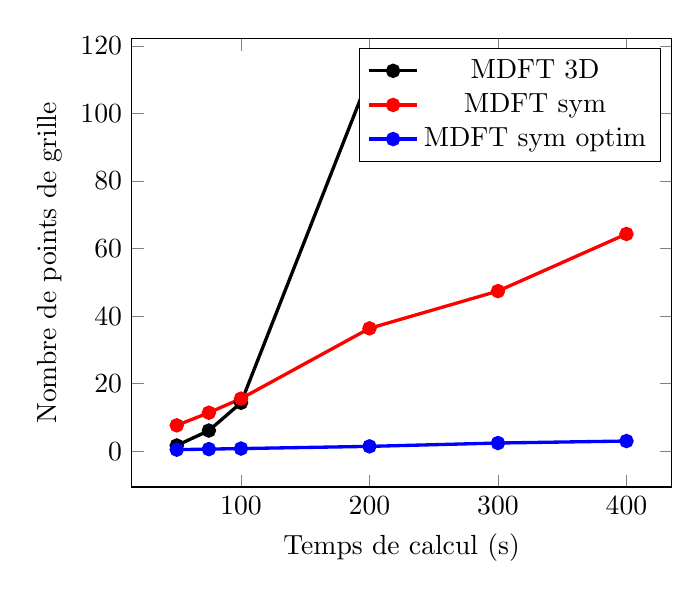
\begin{tikzpicture}
    \begin{axis}[
        xlabel=Temps de calcul (s),
        ylabel=Nombre de points de grille
    ]
    
    \addplot[mark=*, black, very thick] plot coordinates {
        (50,  1.73)
        (75,  6.15)
        (100, 14.37)
        (200, 111.05)
    };
    \addplot[mark=*, red, very thick] plot coordinates {
        (50,  7.69)
        (75,  11.43)
        (100, 15.60)
        (200, 36.39)
        (300, 47.42)
        (400, 64.32)
    };
    \addplot[mark=*, blue, very thick] plot coordinates {
        (50,  0.50)
        (75,  0.66)
        (100, 0.82)
        (200, 1.47)
        (300, 2.46)
        (400, 3.05)
    };


    \legend{MDFT 3D\\MDFT sym\\MDFT sym optim\\}

    \end{axis}
  \end{tikzpicture}
  \caption[Temps de calcul nécessaire à la simulation de la solvatation d'un atome de méthane unifié.]{Temps de calcul nécessaire à la simulation de la solvatation d'un atome de méthane unifié en fonction du nombre de points de grille dans chaque dimension. Le temps nécessaire à la version 3D est représenté en noir, le temps nécessaire à la version à symétrie sphérique sans optimisation est représenté en rouge et avec optimisation en bleu.}
  \label{fig:temps_calcul_methane_versions}
\end{figure}

Il existe bien sur d'autres optimisations possibles comme l'utilisation de transformées de Hankel rapides mais vu le temps de calcul largement convenable, nous avons fait le choix de nous arrêter ici afin de ne pas rendre le code source illisible. Une fois cette version opérationnelle nous avons pu l'utiliser afin de développer notre nouveau bridge.



\section{Le bridge Gros Grain}
A l'aide de la version à symétrie sphérique de la MDFT, nous avons développé un nouveau bridge: le bridge gros grain. Ce bridge doit permettre une amélioration de la prédiction de l'énergie libre de solvatation et des profils de solvant de façon simple et rapide en ajoutant de la consistance thermodynamique au système. Pour cela nous devons, d'une part, reproduire une tension de surface correcte et, d'autre part, corriger la pression du système, qui est largement surestimée dans l'approximation HNC, en rendant possible la coexistence liquide-vapeur. 

\subsection{La tension de surface}
La tension de surface, notée $\gamma$, correspond à l'énergie nécessaire pour créer une unité de surface d'une interface liquide-gaz.

L'énergie libre de solvatation d'une bulle peut être exprimée en fonction de sa surface et de son volume sous la forme:

\begin{equation} \label{eq:energie_libre_terme_volume_surface}
\Delta G_{solv}= \mathrm{A} V_{\mathrm{sphere}} + \gamma S_{\mathrm{sphere}} 
\end{equation}

\noindent Pour des sphères de petits rayons, le terme proportionnelle au volume est prépondérant.
Au contraire, pour les sphères de rayons importants, lorsque leur profils peuvent être assimilés à des murs plats, c'est le terme en surface qui devient prépondérant soit:
\begin{equation}
\lim\limits_{r_{sphere} \to \infty} \Delta G_{solv} = \gamma S_{\mathrm{sphere}} 
\end{equation}
Que l'on réécrit:
\begin{equation}
\lim\limits_{r_{sphere} \to \infty} \frac{\Delta G_{solv}}{S_{\mathrm{sphere}}} = \gamma 
\end{equation}
Le rapport entre l'énergie libre de solvatation et la surface d'une sphère dure de grand diamètre correspond à la tension de surface du solvant, ici de l'eau.
Par la suite nous tracerons donc le rapport entre l'énergie libre de solvatation et la surface des sphères, soit $\frac{\Delta G_{solv}}{S_{\mathrm{sphere}}}$, afin de nous assurer que la tension de surface tend bien vers celle de l'eau.
Nous avons choisi comme référence la tension de surface de l'eau SPC/E et non celle de l'eau réelle afin de rester cohérent avec le modèle utilisé par MDFT.
Comme on l'a montré précédemment, la densité de la phase gazeuse tend vers 0. Pour faciliter le calcul numérique, la bulle de gaz est remplacée par une bulle de vide. Cela revient à faire l'approximation suivante: $\gamma_{liq-gaz} = \gamma_{liq-vide}$



\subsection{Définition du bridge gros grain}
Pour construire notre bridge, nous partons de l'approximation HNC. Cette approximation peut être interprétée comme un développement de Taylor à l'ordre deux de la fonctionnelle d'excès autour de la densité de référence $\rho_{0}$, la densité de l'eau liquide.
Dans cette approximation, comme on le voit sur la figure \ref{fig:fonctionelle_HNC}, plus on s'éloigne de la densité liquide et plus le potentiel chimique du solvant augmente. La phase gaz n'existe donc pas, ce qui à pour conséquence de surestimer fortement la pression du fluide.
Afin de corriger ce phénomène, nous ajoutons un terme d'ordre 3 qui permet de rendre cohérentes les énergies libres de solvatation des deux phases.

D'après la théorie de Landau-Ginzburg\cite{Ginzburg2009}, la hauteur de la courbe entre les deux phases est directement liée à la tension de surface. Nous ajoutons donc un terme d'ordre 4 qui s'annule en $\rho=0$ et $\rho=\rho_0$ afin d'autoriser la modification de cette hauteur sans modifier les deux phases précédemment ajustées.

L'avantage majeur de la MDFT est sa vitesse. Des termes à 3 et 4 corps demanderaient un temps de calcul trop important pour rester concurrentiel par rapport aux méthodes explicites. Afin de rendre le temps de calcul négligeable, nous reprenons une idée de Tarazona et al.\cite{tarazona_free-energy_1985}, qui consiste à remplacer des termes à 3 ou 4 corps par de simples puissances d'ordre 3 et 4 d'une densité gros grain notée $\bar{\rho}(\boldsymbol{r})$ définie comme

\begin{equation} \label{eq:convolution_gros_grain}
\bar{\rho}(\boldsymbol{r}) = \int \mathrm{d}\boldsymbol{r}^\prime \rho(\boldsymbol{r}^\prime) K\left(\left|\boldsymbol{r}-\boldsymbol{r}^\prime\right|\right) = \rho\ast K \left(\boldsymbol{r} \right)
\end{equation}

Le choix du noyau de convolution K sera décrit plus bas. Nous obtenons donc un bridge de la forme suivante:

\begin{equation} \label{eq:fbridge_2}
F_{\mathrm{b}}[\bar{\rho}(\boldsymbol{r})]=A\int\Delta\bar{\rho}(\boldsymbol{r})^3d\boldsymbol{r}+B\int\bar{\rho}(\boldsymbol{r})^2\Delta\bar{\rho}(\boldsymbol{r})^4d\boldsymbol{r}
\end{equation} 


\subsection{\'Etude paramétrique}
A ce niveau, nous disposons d'un bridge que nous pouvons ajuster au travers de 3 paramètres: A, B et le choix du noyau de convolution. Le premier paramètre A est résolu analytiquement de façon à annuler le potentiel chimique de la phase gaz, soit $F[\rho_{liq}]=F[\rho_{gas}]=0$ . Nous obtenons ainsi $A=\mathrm{k_B}T(\frac{1}{\rho_0^2} - \frac{\int c(\boldsymbol{r}) d\boldsymbol{r}}{2\rho_0})$ (en $kJ.mol^{-1}.\text{\AA}^{6}$). Les deux autres paramètres, ont été déterminés à l'aide d'une étude paramétrique.

\subsubsection{Choix du noyau de convolution gros grain}
Il existe différents noyaux de convolutions permettant l'obtention d'une densité gros grain. Notre choix s'est dans un premier temps naturellement porté vers le plus simple, un heavyside (en noir sur la figure \ref{fig:noyaux}). Notre étude a permis d'éliminer rapidement ce noyau de convolution. Il n'existait aucune combinaison de paramètres permettant de reproduire correctement la tension de surface (résultats non présentés ici). 










\pgfmathdeclarefunction{gauss}{2}{%
    \pgfmathparse{1/(#2*sqrt(2*pi))*exp(-((x-#1)^2)/(2*#2^2))}%
}

\begin{figure}[ht]
    \center    
  \begin{tikzpicture}
    \begin{axis}[
            xlabel= distance (\AA),
%            ylabel= $\Delta g$ (kJ/mol/\AA$^3$),
            xmin = -2, xmax = 2,
            ymin = 0, ymax = 2,
            no markers,
            legend style = {draw = none, cells={anchor=west}}
      ]
      \addplot[mark=none, black, very thick] plot coordinates {
        (-2,  0)
        (-1,  0)
        (-1,  0.5)
        (1,  0.5)
        (1, 0)
        (2, 0)
     };
      
      \addplot[mark=none, red, very thick, domain=-2:2, samples=400] {gauss(0,0.3)};
      \legend{heavyside, gaussienne}
    \end{axis}
  \end{tikzpicture}
    \caption[Noyaux de convolution utilisés dans l'étude paramétrique permettant la définition du bridge gros grain.]{Noyaux de convolution utilisés dans l'étude paramétrique permettant la définition du bridge gros grain. En noir le heavyside et en rouge la gaussienne.}
    \label{fig:noyaux}
\end{figure}



Nous nous sommes ensuite intéressés à la gaussienne (en rouge sur la figure \ref{fig:noyaux}).
Ce noyau est défini par deux paramètres, sa largeur à mi hauteur $\sigma_{gauss}$ (\AA) et un pré-facteur définissant sa hauteur.
Afin de conserver une cohérence entre la densité et la densité gros grain, le pré-facteur est choisi de façon à obtenir une aire sous la courbe de la gaussienne toujours égale à 1.
\`A ce niveau, nous disposons donc de deux paramètres, B et $\sigma_{gauss}$.
Dans un premier temps, nous avons cherché les limites de B qui ont un impact direct sur la forme de la courbe de potentiel chimique du fluide homogène.
Comme on le voit sur la figure \ref{fig:etude_B}, une valeur de B inférieure à $-15e^{-8}\  \mathrm{kJ.mol}^{-1}.\text{\AA}^{15}$ ou supérieure à $15e^{-8} \mathrm{kJ.mol}^{-1}.\text{\AA}^{15}$ déforme la courbe.
Nous avons donc choisi de concentrer notre étude sur des valeurs de B allant de $-15e^{-8}$ à $15e^{-8} \mathrm{kJ.mol}^{-1}.\text{\AA}^{15}$.
La figure \ref{fig:etude_B_zoom} correspond à un zoom de la fonctionnelle autour de l'origine. On voit la création d'un second minimum proche de zero qui confirme la présence d'une phase gazeuse. On voit également que le minimum est très légèrement négatif. Ce résultat est attendu car on impose $\rho[0]=0$ et on sait que $\frac{\delta F}{\delta \rho}<0$ (voir annexe \ref{chap:annexes:grad}).

\begin{figure}[ht]
    \center
  \begin{tikzpicture}
    \begin{axis}[
           xlabel= $\rho_{bulk}/\rho_0$,
            ylabel= $\Delta g_{solv} (kJ.mol^{-1}.\text{\AA}^{-3}) $,
            xmin = 0, xmax = 1.5,
            ymin = 0, ymax = 0.15,
            scaled y ticks={base 10:2},
            legend style = {draw = none, cells={anchor=west}}
      ]
      \addplot+[mark=none, very thick] file {chapters/bridge/datas/fonctionnelles/fonctionnelle_-15.0.csv};
      \addplot+[mark=none, very thick] file {chapters/bridge/datas/fonctionnelles/fonctionnelle_-10.0.csv};
      \addplot+[mark=none, very thick] file {chapters/bridge/datas/fonctionnelles/fonctionnelle_-5.0.csv};
      \addplot+[mark=none, very thick] file {chapters/bridge/datas/fonctionnelles/fonctionnelle_0.0.csv};
      \addplot+[mark=none, very thick] file {chapters/bridge/datas/fonctionnelles/fonctionnelle_5.0.csv};
      \addplot+[mark=none, very thick] file {chapters/bridge/datas/fonctionnelles/fonctionnelle_10.0.csv};
      \addplot+[mark=none, very thick] file {chapters/bridge/datas/fonctionnelles/fonctionnelle_15.0.csv};
      \legend{$B=-15$, $B=-10$, $B=-5$, $B=0$, $B=5$, $B=10$, $B=15$}
    \end{axis}
  \end{tikzpicture}
    \caption[\'Energie libre d'une unité de volume du solvant homogène en fonction du paramètre B.]{\'Energie libre d'une unité de volume du solvant homogène de densité $\rho_\mathrm{bulk}$ en fonction du paramètre B ($e^{-8} \mathrm{kJ.mol}^{-1}.\text{\AA}^{15}$). $\rho_0$ est la densité bulk de l'eau SPC/E à pression et température standards (1$kg.L^{-1}$).}
    \label{fig:etude_B}
\end{figure}


\begin{figure}[ht]
    \center
  \begin{tikzpicture}
    \begin{axis}[
           xlabel= $\rho_{bulk}/\rho_0$,
            ylabel= $\Delta g_{solv} (kJ.mol^{-1}.\text{\AA}^{-3}) $,
            scaled x ticks={base 10:0},
            scaled y ticks={base 10:0},
            xtick = {0, 0.0001, 0.0002},
			xmin = 0, xmax = 0.0002,
            legend style = {draw = none, cells={anchor=west}}
      ]
      \addplot+[mark=none, very thick] file {chapters/bridge/datas/fonctionnelles/fonctionnelle_0.0_zoom.csv};
      \addplot[mark=none, dashed, black, very thick] coordinates { (0, 0) (0.0002, 0) };
    \end{axis}
  \end{tikzpicture}
    \caption[Zoom de l'\'energie libre d'une unité de volume du solvant homogène autour de l'origine.]{Zoom de l'\'energie libre d'une unité de volume du solvant homogène autour de l'origine. On observe un nouveau minimum correspondant à la phase gazeuse du solvant.}
    \label{fig:etude_B_zoom}
\end{figure}


\subsubsection{\'Exploration des paramètres B et $\sigma_{gauss}$}
Pour chaque valeur de ce paramètre B, nous avons tracé l'énergie libre de solvatation d'une sphère dure divisée par son volume en fonction de son rayon.
Nous avons ensuite ajusté la valeur de $\sigma_{gauss}$ pour obtenir une tension de surface correcte (voir figure \ref{fig:etude_sigma}).

\begin{figure}[ht]
\center
    \begin{tikzpicture}
      \begin{axis}[
          xlabel= $R$ (\AA),
          ylabel= $\Delta G_{\textrm{solv}}/(4\pi R^2)$ (mJ/m$^2$), 
          xmin = 0, xmax = 100,
          ymin = 0, ymax = 80,
          legend style = {draw = none, at={(0.95,0.05)},anchor=south east}%,
          ]
        \addplot+[mark=none, very thick] table[x index=0, y index=4] {chapters/bridge/datas/free_energy_by_volume/results_HS_0.866_15.csv};
        \addplot+[mark=none, very thick] table[x index=0, y index=4] {chapters/bridge/datas/free_energy_by_volume/results_HS_0.900_15.csv};
        \addplot+[mark=none, very thick] table[x index=0, y index=4] {chapters/bridge/datas/free_energy_by_volume/results_HS_0.935_15.csv};
        \addplot+[mark=none, very thick] table[x index=0, y index=4] {chapters/bridge/datas/free_energy_by_volume/results_HS_0.966_15.csv};
        \addplot+[mark=none, very thick] table[x index=0, y index=4] {chapters/bridge/datas/free_energy_by_volume/results_HS_1.000_15.csv};
        \addplot[mark=none, dashed, black, very thick] coordinates { (0, 63.6) (100, 63.6) };
        \legend{$\sigma_{gauss}=0.866$, $\sigma_{gauss}=0.900$, $\sigma_{gauss}=0.935$, $\sigma_{gauss}=0.966$, $\sigma_{gauss}=1.000$}
      \end{axis}
    \end{tikzpicture}
	\caption[\'Energie libre de solvatation d'une sphère dure divisée par sa surface en fonction de son rayon  pour différentes valeurs de $\sigma_{gauss}$.]{\'Energie libre de solvatation d'une sphère dure divisée par sa surface en fonction de son rayon  pour différentes valeurs de $\sigma_{gauss}$ (en \AA), largeur de la gaussienne servant à la convolution. B est fixé ici à $15e^{-8} kJ.mol^{-1}.\text{\AA}^{15}$. La valeur de référence en pointillé est la valeur de la tension de surface de l'eau SPC/E soit 63.3 mJ.m$^{-2}$\cite{vega_surface_2007}.}
    \label{fig:etude_sigma}
\end{figure}


Nous avons ainsi obtenu, pour chaque valeur de B sélectionnée, la valeur de $\sigma_{gauss}$ reproduisant correctement la tension de surface $\gamma$ de l'eau. Ces valeurs sont disponibles dans le tableau \ref{tab:parametres_bridge}.

\begin{table}[ht]
 \centering
  \begin{tabular}{l || c c c c c c c}
    \hline
    B ($e^{-8} \mathrm{kJ.mol}^{-1}.\text{\AA}^{15}$)  & -15 & -10 & -5 & 0 & 5 & 10 & 15  \\
    \hline
     $\sigma_{gauss}$ (\AA)  & 1.177 & 1.110 & 1.061 & 1.021 & 0.989 & 0.960 & 0.935  \\
    \hline
  \end{tabular}
  \caption{Couples de paramètres permettant d'obtenir la bonne tension de surface de l'eau.}
  \label{tab:parametres_bridge}  
\end{table}

Afin de sélectionner le meilleur couple de paramètres, nous disposons de différentes références, que ce soit de structure de solvant ou d'énergie libre de solvatation. 

%!!!!!!!!!!!!!!!!!!!!!!!!!!!!!!!!!!!!!!!!!!!!!!!!!
%\begin{figure}[H]
%    \center    
%  \begin{tikzpicture}
%    \begin{axis}[
%            xlabel= $\rho$/$\rho_b$,
%            ylabel= $\Delta g$ (kJ/mol/\AA$^3$),
%            legend style = {draw = none, cells={anchor=west}}
%      ]
%      \addplot+[mark=none, very thick] plot coordinates {
%        (-15, 1.177)
%        (-10, 1.110)
%        (-5,  1.061)
%        (0,   1.021)
%        (5,   0.989)
%        (10,  0.960)
%        (15,  0.935)
%     };
%    \end{axis}
%  \end{tikzpicture}
%    \caption{}}
%    \label{fig:parametres_b_sigma}
%\end{figure}
%!!!!!!!!!!!!!!!!!!!!!!!!!!!!!!!!!!!!!!!!!!!!!!!!!!

\subsubsection{\'Energie libre de solvatation de sphères dures}
Dans un premier temps, nous comparons, pour chaque jeu de paramètres, l'\'energie libre de solvatation d'une sphère dure divisée par sa surface aux valeurs de références calculées par Monte Carlo\cite{hummer_information_1996} (voir figure \ref{fig:comparaison_hummer}). A cause du temps de calcul nécessaire, Hummer et al\cite{hummer_information_1996}, se sont limités à une dizaine de point pour des sphères de rayon inférieur à 4 \AA.



\begin{sidewaysfigure}
\begin{figure}[H]
\centering
\begin{subfigure}{.24\textwidth}
  \centering
    \caption{HNC}
    \resizebox{\linewidth}{!}{
    \begin{tikzpicture}
        	\begin{axis}[
                xlabel= $R$ (\AA),
          		ylabel= $\Delta G_{\textrm{solv}}/(4\pi R^2)$ (mJ/m$^2$), 
    	        restrict x to domain=0:5,
    	        restrict y to domain=0:50,
            	xmin = 0,
        	    xmax = 4,
                ymin = 0,
	            ymax = 40,
        	    legend style = {draw = none, cells={anchor=west}}%,
               % xmode=log
    	        ]
            	\addplot+[mark=none, red, very thick] table[x index=0, y index=2]{chapters/bridge/datas/free_energy_by_volume/results_HS_HNC.csv};
                \addplot+[only marks,mark=*,mark options={scale=1.3, black, fill=black},text mark as node=true] table[x index=0, y index=1] {chapters/bridge/datas/free_energy_by_volume/hummer_ref.csv};
        	\end{axis}
    \end{tikzpicture}
  }
  \end{subfigure}
\begin{subfigure}{.24\textwidth}
  \centering
    \caption{B=15, $\sigma_{gauss}$=0.935}
    \resizebox{\linewidth}{!}{
    \begin{tikzpicture}
        	\begin{axis}[
                xlabel= $R$ (\AA),
          		ylabel= $\Delta G_{\textrm{solv}}/(4\pi R^2)$ (mJ/m$^2$), 
    	        restrict x to domain=0:5,
    	        restrict y to domain=0:50,
            	xmin = 0,
        	    xmax = 4,
                ymin = 0,
	            ymax = 40,
        	    legend style = {draw = none, cells={anchor=west}}%,
               % xmode=log
    	        ]
            	\addplot+[mark=none, red, very thick] table[x index=0, y index=2]{chapters/bridge/datas/free_energy_by_volume/results_HS_0.935_15.csv};
                \addplot+[only marks,mark=*,mark options={scale=1.3, black, fill=black},text mark as node=true] table[x index=0, y index=1] {chapters/bridge/datas/free_energy_by_volume/hummer_ref.csv};
        	\end{axis}
    \end{tikzpicture}
  }
  \end{subfigure}
\begin{subfigure}{.24\textwidth}
  \centering
    \caption{B=10, $\sigma_{gauss}$=0.960}
    \resizebox{\linewidth}{!}{
    \begin{tikzpicture}
        	\begin{axis}[
                xlabel= $R$ (\AA),
          		ylabel= $\Delta G_{\textrm{solv}}/(4\pi R^2)$ (mJ/m$^2$), 
    	        restrict x to domain=0:5,
    	        restrict y to domain=0:50,
            	xmin = 0,
        	    xmax = 4,
                ymin = 0,
	            ymax = 40,
        	    legend style = {draw = none, cells={anchor=west}}%,
               % xmode=log
    	        ]
            	\addplot+[mark=none, red, very thick] table[x index=0, y index=2]{chapters/bridge/datas/free_energy_by_volume/results_HS_0.960_10.csv};
                \addplot+[only marks,mark=*,mark options={scale=1.3, black, fill=black},text mark as node=true] table[x index=0, y index=1] {chapters/bridge/datas/free_energy_by_volume/hummer_ref.csv};
        	\end{axis}
    \end{tikzpicture}
  }
  \end{subfigure}
\begin{subfigure}{.24\textwidth}
  \centering
    \caption{B=5, $\sigma_{gauss}$=0.989}
    \resizebox{\linewidth}{!}{
    \begin{tikzpicture}
        	\begin{axis}[
                xlabel= $R$ (\AA),
          		ylabel= $\Delta G_{\textrm{solv}}/(4\pi R^2)$ (mJ/m$^2$), 
    	        restrict x to domain=0:5,
    	        restrict y to domain=0:50,
            	xmin = 0,
        	    xmax = 4,
                ymin = 0,
	            ymax = 40,
        	    legend style = {draw = none, cells={anchor=west}}%,
               % xmode=log
    	        ]
            	\addplot+[mark=none, red, very thick] table[x index=0, y index=2]{chapters/bridge/datas/free_energy_by_volume/results_HS_0.989_5.csv};
                \addplot+[only marks,mark=*,mark options={scale=1.3, black, fill=black},text mark as node=true] table[x index=0, y index=1] {chapters/bridge/datas/free_energy_by_volume/hummer_ref.csv};
        	\end{axis}
    \end{tikzpicture}
  }
  \end{subfigure}
\begin{subfigure}{.24\textwidth}
  \centering
    \caption{B=0, $\sigma_{gauss}$=1.021}
    \resizebox{\linewidth}{!}{
    \begin{tikzpicture}
        	\begin{axis}[
                xlabel= $R$ (\AA),
          		ylabel= $\Delta G_{\textrm{solv}}/(4\pi R^2)$ (mJ/m$^2$), 
    	        restrict x to domain=0:5,
    	        restrict y to domain=0:50,
            	xmin = 0,
        	    xmax = 4,
                ymin = 0,
	            ymax = 40,
        	    legend style = {draw = none, cells={anchor=west}}%,
               % xmode=log
    	        ]
            	\addplot+[mark=none, red, very thick] table[x index=0, y index=2]{chapters/bridge/datas/free_energy_by_volume/results_HS_1.021_0.csv};
                \addplot+[only marks,mark=*,mark options={scale=1.3, black, fill=black},text mark as node=true] table[x index=0, y index=1] {chapters/bridge/datas/free_energy_by_volume/hummer_ref.csv};
        	\end{axis}
    \end{tikzpicture}
  }
  \end{subfigure}
\begin{subfigure}{.24\textwidth}
  \centering
    \caption{B=-5, $\sigma_{gauss}$=1.061}
    \resizebox{\linewidth}{!}{
    \begin{tikzpicture}
        	\begin{axis}[
                xlabel= $R$ (\AA),
          		ylabel= $\Delta G_{\textrm{solv}}/(4\pi R^2)$ (mJ/m$^2$), 
    	        restrict x to domain=0:5,
    	        restrict y to domain=0:50,
            	xmin = 0,
        	    xmax = 4,
                ymin = 0,
	            ymax = 40,
        	    legend style = {draw = none, cells={anchor=west}}%,
               % xmode=log
    	        ]
            	\addplot+[mark=none, red, very thick] table[x index=0, y index=2]{chapters/bridge/datas/free_energy_by_volume/results_HS_1.061_-5.csv};
                \addplot+[only marks,mark=*,mark options={scale=1.3, black, fill=black},text mark as node=true] table[x index=0, y index=1] {chapters/bridge/datas/free_energy_by_volume/hummer_ref.csv};
        	\end{axis}
    \end{tikzpicture}
  }
  \end{subfigure}
\begin{subfigure}{.24\textwidth}
  \centering
    \caption{B=-10, $\sigma_{gauss}$=1.110}
    \resizebox{\linewidth}{!}{
    \begin{tikzpicture}
        	\begin{axis}[
                xlabel= $R$ (\AA),
          		ylabel= $\Delta G_{\textrm{solv}}/(4\pi R^2)$ (mJ/m$^2$), 
    	        restrict x to domain=0:5,
    	        restrict y to domain=0:50,
            	xmin = 0,
        	    xmax = 4,
                ymin = 0,
	            ymax = 40,
        	    legend style = {draw = none, cells={anchor=west}}%,
               % xmode=log
    	        ]
            	\addplot+[mark=none, red, very thick] table[x index=0, y index=2]{chapters/bridge/datas/free_energy_by_volume/results_HS_1.110_-10.csv};
                \addplot+[only marks,mark=*,mark options={scale=1.3, black, fill=black},text mark as node=true] table[x index=0, y index=1] {chapters/bridge/datas/free_energy_by_volume/hummer_ref.csv};
        	\end{axis}
    \end{tikzpicture}
  }
  \end{subfigure}
\begin{subfigure}{.24\textwidth}
  \centering
    \caption{B=-15, $\sigma_{gauss}$=1.177}
    \resizebox{\linewidth}{!}{
    \begin{tikzpicture}
        	\begin{axis}[
                xlabel= $R$ (\AA),
          		ylabel= $\Delta G_{\textrm{solv}}/(4\pi R^2)$ (mJ/m$^2$), 
    	        restrict x to domain=0:5,
    	        restrict y to domain=0:50,
            	xmin = 0,
        	    xmax = 4,
                ymin = 0,
	            ymax = 40,
        	    legend style = {draw = none, cells={anchor=west}}%,
               % xmode=log
    	        ]
            	\addplot+[mark=none, red, very thick] table[x index=0, y index=2]{chapters/bridge/datas/free_energy_by_volume/results_HS_1.177_-15.csv};
                \addplot+[only marks,mark=*,mark options={scale=1.3, black, fill=black},text mark as node=true] table[x index=0, y index=1] {chapters/bridge/datas/free_energy_by_volume/hummer_ref.csv};
        	\end{axis}
    \end{tikzpicture}
  }
  \end{subfigure}
    \caption[\'Energie libre de solvatation d'une sphère dure divisée par sa surface en fonction de son rayon pour différentes valeurs de B.]{ \'Energie libre de solvatation d'une sphère dure divisée par sa surface en fonction de son rayon calculée dans l'approximation HNC puis avec les différents paramètres du bridge. Les calculs ont été effectués pour chaque couple de paramètres B ($e^{-8} \mathrm{kJ.mol}^{-1}.\text{\AA}^{15}$) et $\sigma_{gauss}$ (\AA). Ces courbes en rouge, sont comparés à des valeurs de référence (sphères noires) calculées par Monte-Carlo\cite{hummer_information_1996} }
    \label{fig:comparaison_hummer}
\end{figure}
\end{sidewaysfigure}


 On voit que l'approximation HNC, surestime les énergies libres de solvatation. Notre bridge, corrige fortement cet écart, quelque soit le couple de paramètre choisi. Les meilleurs paramètres ici semblent être pour un B autour de $5e^{-8}\  \mathrm{kJ.mol}^{-1}.\text{\AA}^{15}$. 

\boitesimple{Les \'energies libres de solvatation de sphères dures les plus précises sont obtenus pour un B autour de $5e^{-8}\  \mathrm{kJ.mol}^{-1}.\text{\AA}^{15}$. Chacun des paramètres proposés sont acceptables à ce niveau. }
 



\subsubsection{\'Energie libre de solvatation de molécules modèles}
Nous avons ensuite calculé l'énergie libre de solvatation de molécules modèles avec MDFT, pour les différents paramètres du bridge, et par dynamique moléculaire. Nos molécules modèles sont le méthane unifié et les gaz rares: Néon, Argon, Krypton, Xénon. L'ensemble de ces résultats est disponible dans le tableau \ref{tab:energie_libre_molecules_models}. Les paramètres Lennard-Jones de ces composés sont disponibles dans le tableau \ref{tab:param_lj}.


\begin{table}[ht]
  \centering
  \begin{tabular}{ l c c c c c c c c c c c }
   \hline & \\[-1em]\hline
    Méthode    & Exp   & DM    & HNC    &      &       &       & MDFT  &       &       & \\
    \hline
    B          &       &       &        & -15   & -10   & -5    & 0     & 5     & 10    & 15     \\
    $\sigma_{gauss}$   &       &       &        & 1.177 & 1.110 & 1.061 & 1.021 & 0.989 & 0.960 & 0.935  \\
    \hline
    Méthane    &       &  9.23 & 28.14  & 15.97 & 14.55 & 13.70 & 13.05 & 12.62 & 12.25 & \textbf{11.99}  \\
%    Neopentane &       &  0.37 & 84.51 & 17.51 & 13.77 & 11.30 &  9.43 &  8.17 &  7.05 &  \textbf{6.23}  \\
    Néon       & 10.36 & 11.73 & 19.04  & 14.89 & 14.25 & 13.83 & 13.53 & 13.34 & 13.19 & \textbf{13.10}  \\
    Argon      &  8.40 &  8.61 & 22.89  & 14.16 & 13.12 & 12.42 & 11.89 & 11.55 & 11.25 & \textbf{11.01}  \\
    Krypton    &  6.96 &  8.03 & 26.41  & 14.54 & 13.28 & 12.44 & 11.80 & 11.38 & 11.00 & \textbf{10.74}  \\
    Xénon       &  6.06 &  6.47 & 31.23 & 15.02 & 13.50 & 12.48 & 11.71 & 11.20 & 10.74 & \textbf{10.33}  \\
    \hline & \\[-1em]\hline
  \end{tabular}
  \caption[\'Energie libre de solvatation du méthane unifié et des gaz rares.]{Valeurs de l'énergie libre de solvatation (en kJ.mol$^{-1}$) du méthane unifié et des gaz rares: Argon, Xénon, Krypton, Néon pour les différents paramètres possibles de la fonctionnelle de bridge gros grain. Les valeurs les plus proches de notre référence, la dynamique moléculaire, sont en gras.}
  \label{tab:energie_libre_molecules_models}  
\end{table}


\begin{table}[ht]
  \centering
  \begin{tabular}{ l c c }
   \hline & \\[-1em]\hline
    Méthode    & $\sigma_{LJ}$ (\AA) & $\epsilon_{LJ}$ (kJ.mol$^{-1}$) \\
    \hline
      méthane & 3.73000 & 1.2300 \\
	  néon & 3.03500 & 0.15432 \\
	  argon & 3.41500 & 1.03931 \\
	  krypton & 3.67500 & 1.4051 \\
	  xenon & 3.97500 & 1.7851 \\
    \hline & \\[-1em]\hline
  \end{tabular}
  \caption[Paramètres Lennard-Jones du méthane unifié et des gaz rares utilisés dans nos simulations.]{Paramètres Lennard-Jones du méthane unifié et des gaz rares utilisés dans nos simulations.}
  \label{tab:param_lj}  
\end{table}


On remarque que l'approximation HNC surestime fortement le calcul de l'énergie libre de solvatation de plusieurs dizaines de $\mathrm{kJ.mol}^{-1}$. Le bridge gros grain permet de considérablement réduire cet écart, à quelques $\mathrm{kJ.mol}^{-1}$ seulement.
On remarque également que plus B est grand et donc plus la barrière de transition entre la phase liquide et gaz est importante, et meilleures sont les prédictions d'énergies libres de solvatation. 

\boitesimple{ Les meilleures énergies libres de solvatation de nos molécules modèles sont obtenues avec B=$15e^{-8}\  \mathrm{kJ.mol}^{-1}.\text{\AA}^{15}$  et $\sigma_{gauss}$ = 0.935 \AA }



\subsubsection{ Structure du solvant autour de sphères dures }
Nous nous sommes également intéressés aux structures de solvant, dans un premier temps, autour de sphère dures (voir figure \ref{fig:g_r_HS}). Les profils calculés pour chacun des paramètres ont été comparés à des profils de références calculés par Monte Carlo et publiés par Chandler et al.\cite{huang_hydrophobic_2002}. \'Etant donné les temps de calcul nécessaires à la production de ces références, ils se sont limités à des sphères dures de 2, 4, 6, 8 et 10 \AA.




\begin{sidewaysfigure}
\begin{figure}[H]
\centering
\begin{subfigure}{.24\textwidth}
  \centering
    \caption{HNC}
    \resizebox{\linewidth}{!}{
      \begin{tikzpicture}
          \begin{axis}[
              xlabel= r ($\text{\AA}$),
              ylabel= g(r),
              xmin = 0,
              xmax = 16,
              ymin = 0,
              ymax = 8,
              legend style = {draw = none, cells={anchor=west}}
              ]
              \addplot+[mark=none, black, very thick, solid] table[x index=0,y index=1] {chapters/bridge/datas/g_of_r/data_HS_HNC/g_HS_HNC_2_4_6_8_10.csv};
              \addplot+[mark=none, blue, very thick, dashed] file {chapters/bridge/datas/g_of_r/chandler_ref/chandler_2.csv};
              \addplot+[mark=none, black, very thick, solid] table[x index=0,y index=2] {chapters/bridge/datas/g_of_r/data_HS_HNC/g_HS_HNC_2_4_6_8_10.csv};
              \addplot+[mark=none, blue, very thick, dashed] file {chapters/bridge/datas/g_of_r/chandler_ref/chandler_4.csv};
              \addplot+[mark=none, black, very thick, solid] table[x index=0,y index=3] {chapters/bridge/datas/g_of_r/data_HS_HNC/g_HS_HNC_2_4_6_8_10.csv};
              \addplot+[mark=none, blue, very thick, dashed] file {chapters/bridge/datas/g_of_r/chandler_ref/chandler_6.csv};
              \addplot+[mark=none, black, very thick, solid] table[x index=0,y index=4] {chapters/bridge/datas/g_of_r/data_HS_HNC/g_HS_HNC_2_4_6_8_10.csv};
              \addplot+[mark=none, blue, very thick, dashed] file {chapters/bridge/datas/g_of_r/chandler_ref/chandler_8.csv};
              \addplot+[mark=none, black, very thick, solid] table[x index=0,y index=5] {chapters/bridge/datas/g_of_r/data_HS_HNC/g_HS_HNC_2_4_6_8_10.csv};
              \addplot+[mark=none, blue, very thick, dashed] file {chapters/bridge/datas/g_of_r/chandler_ref/chandler_10.csv};
              \legend{ MDFT(HNC), MC}
          \end{axis}
      \end{tikzpicture}
    }
  \end{subfigure}
\begin{subfigure}{.24\textwidth}
  \centering
    \caption{B=15, $\sigma_{gauss}$=0.935}
    \resizebox{\linewidth}{!}{
      \begin{tikzpicture}
          \begin{axis}[
              xlabel= r ($\text{\AA}$),
              ylabel= g(r),
              xmin = 0,
              xmax = 16,
              ymin = 0,
              ymax = 8,
              legend style = {draw = none, cells={anchor=west}}
              ]
              \addplot+[mark=none, red, very thick, solid] table[x index=0,y index=1] {chapters/bridge/datas/g_of_r/data_HS_HNC_bridge_0.935_15/g_HS_HNC_bridge_2_4_6_8_10.csv};
              \addplot+[mark=none, blue, very thick, dashed] file {chapters/bridge/datas/g_of_r/chandler_ref/chandler_2.csv};
              \addplot+[mark=none, red, very thick, solid] table[x index=0,y index=2] {chapters/bridge/datas/g_of_r/data_HS_HNC_bridge_0.935_15/g_HS_HNC_bridge_2_4_6_8_10.csv};
              \addplot+[mark=none, blue, very thick, dashed] file {chapters/bridge/datas/g_of_r/chandler_ref/chandler_4.csv};
              \addplot+[mark=none, red, very thick, solid] table[x index=0,y index=3] {chapters/bridge/datas/g_of_r/data_HS_HNC_bridge_0.935_15/g_HS_HNC_bridge_2_4_6_8_10.csv};
              \addplot+[mark=none, blue, very thick, dashed] file {chapters/bridge/datas/g_of_r/chandler_ref/chandler_6.csv};
              \addplot+[mark=none, red, very thick, solid] table[x index=0,y index=4] {chapters/bridge/datas/g_of_r/data_HS_HNC_bridge_0.935_15/g_HS_HNC_bridge_2_4_6_8_10.csv};
              \addplot+[mark=none, blue, very thick, dashed] file {chapters/bridge/datas/g_of_r/chandler_ref/chandler_8.csv};
              \addplot+[mark=none, red, very thick, solid] table[x index=0,y index=5] {chapters/bridge/datas/g_of_r/data_HS_HNC_bridge_0.935_15/g_HS_HNC_bridge_2_4_6_8_10.csv};
              \addplot+[mark=none, blue, very thick, dashed] file {chapters/bridge/datas/g_of_r/chandler_ref/chandler_10.csv};
              \legend{MDFT(HNC+B), MC}
          \end{axis}
      \end{tikzpicture}
    }
  \end{subfigure}
\begin{subfigure}{.24\textwidth}
  \centering
    \caption{B=10, $\sigma_{gauss}$=0.960}
    \resizebox{\linewidth}{!}{
      \begin{tikzpicture}
          \begin{axis}[
              xlabel= r ($\text{\AA}$),
              ylabel= g(r),
              xmin = 0,
              xmax = 16,
              ymin = 0,
              ymax = 8,
              legend style = {draw = none, cells={anchor=west}}
              ]
              \addplot+[mark=none, red, very thick, solid] table[x index=0,y index=1] {chapters/bridge/datas/g_of_r/data_HS_HNC_bridge_0.960_10/g_HS_HNC_bridge_2_4_6_8_10.csv};
              \addplot+[mark=none, blue, very thick, dashed] file {chapters/bridge/datas/g_of_r/chandler_ref/chandler_2.csv};
              \addplot+[mark=none, red, very thick, solid] table[x index=0,y index=2] {chapters/bridge/datas/g_of_r/data_HS_HNC_bridge_0.960_10/g_HS_HNC_bridge_2_4_6_8_10.csv};
              \addplot+[mark=none, blue, very thick, dashed] file {chapters/bridge/datas/g_of_r/chandler_ref/chandler_4.csv};
              \addplot+[mark=none, red, very thick, solid] table[x index=0,y index=3] {chapters/bridge/datas/g_of_r/data_HS_HNC_bridge_0.960_10/g_HS_HNC_bridge_2_4_6_8_10.csv};
              \addplot+[mark=none, blue, very thick, dashed] file {chapters/bridge/datas/g_of_r/chandler_ref/chandler_6.csv};
              \addplot+[mark=none, red, very thick, solid] table[x index=0,y index=4] {chapters/bridge/datas/g_of_r/data_HS_HNC_bridge_0.960_10/g_HS_HNC_bridge_2_4_6_8_10.csv};
              \addplot+[mark=none, blue, very thick, dashed] file {chapters/bridge/datas/g_of_r/chandler_ref/chandler_8.csv};
              \addplot+[mark=none, red, very thick, solid] table[x index=0,y index=5] {chapters/bridge/datas/g_of_r/data_HS_HNC_bridge_0.960_10/g_HS_HNC_bridge_2_4_6_8_10.csv};
              \addplot+[mark=none, blue, very thick, dashed] file {chapters/bridge/datas/g_of_r/chandler_ref/chandler_10.csv};
              \legend{MDFT(HNC+B), MC}
          \end{axis}
      \end{tikzpicture}
    }
  \end{subfigure}
\begin{subfigure}{.24\textwidth}
  \centering
    \caption{B=5, $\sigma_{gauss}$=0.989}
    \resizebox{\linewidth}{!}{
      \begin{tikzpicture}
          \begin{axis}[
              xlabel= r ($\text{\AA}$),
              ylabel= g(r),
              xmin = 0,
              xmax = 16,
              ymin = 0,
              ymax = 8,
              legend style = {draw = none, cells={anchor=west}}
              ]
              \addplot+[mark=none, red, very thick, solid] table[x index=0,y index=1] {chapters/bridge/datas/g_of_r/data_HS_HNC_bridge_0.989_5/g_HS_HNC_bridge_2_4_6_8_10.csv};
              \addplot+[mark=none, blue, very thick, dashed] file {chapters/bridge/datas/g_of_r/chandler_ref/chandler_2.csv};
              \addplot+[mark=none, red, very thick, solid] table[x index=0,y index=2] {chapters/bridge/datas/g_of_r/data_HS_HNC_bridge_0.989_5/g_HS_HNC_bridge_2_4_6_8_10.csv};
              \addplot+[mark=none, blue, very thick, dashed] file {chapters/bridge/datas/g_of_r/chandler_ref/chandler_4.csv};
              \addplot+[mark=none, red, very thick, solid] table[x index=0,y index=3] {chapters/bridge/datas/g_of_r/data_HS_HNC_bridge_0.989_5/g_HS_HNC_bridge_2_4_6_8_10.csv};
              \addplot+[mark=none, blue, very thick, dashed] file {chapters/bridge/datas/g_of_r/chandler_ref/chandler_6.csv};
              \addplot+[mark=none, red, very thick, solid] table[x index=0,y index=4] {chapters/bridge/datas/g_of_r/data_HS_HNC_bridge_0.989_5/g_HS_HNC_bridge_2_4_6_8_10.csv};
              \addplot+[mark=none, blue, very thick, dashed] file {chapters/bridge/datas/g_of_r/chandler_ref/chandler_8.csv};
              \addplot+[mark=none, red, very thick, solid] table[x index=0,y index=5] {chapters/bridge/datas/g_of_r/data_HS_HNC_bridge_0.989_5/g_HS_HNC_bridge_2_4_6_8_10.csv};
              \addplot+[mark=none, blue, very thick, dashed] file {chapters/bridge/datas/g_of_r/chandler_ref/chandler_10.csv};
              \legend{MDFT(HNC+B), MC}
          \end{axis}
      \end{tikzpicture}
    }
  \end{subfigure}
\begin{subfigure}{.24\textwidth}
  \centering
    \caption{B=0, $\sigma_{gauss}$=1.021}
    \resizebox{\linewidth}{!}{
      \begin{tikzpicture}
          \begin{axis}[
              xlabel= r ($\text{\AA}$),
              ylabel= g(r),
              xmin = 0,
              xmax = 16,
              ymin = 0,
              ymax = 8,
              legend style = {draw = none, cells={anchor=west}}
              ]
              \addplot+[mark=none, red, very thick, solid] table[x index=0,y index=1] {chapters/bridge/datas/g_of_r/data_HS_HNC_bridge_1.021_0/g_HS_HNC_bridge_2_4_6_8_10.csv};
              \addplot+[mark=none, blue, very thick, dashed] file {chapters/bridge/datas/g_of_r/chandler_ref/chandler_2.csv};
              \addplot+[mark=none, red, very thick, solid] table[x index=0,y index=2] {chapters/bridge/datas/g_of_r/data_HS_HNC_bridge_1.021_0/g_HS_HNC_bridge_2_4_6_8_10.csv};
              \addplot+[mark=none, blue, very thick, dashed] file {chapters/bridge/datas/g_of_r/chandler_ref/chandler_4.csv};
              \addplot+[mark=none, red, very thick, solid] table[x index=0,y index=3] {chapters/bridge/datas/g_of_r/data_HS_HNC_bridge_1.021_0/g_HS_HNC_bridge_2_4_6_8_10.csv};
              \addplot+[mark=none, blue, very thick, dashed] file {chapters/bridge/datas/g_of_r/chandler_ref/chandler_6.csv};
              \addplot+[mark=none, red, very thick, solid] table[x index=0,y index=4] {chapters/bridge/datas/g_of_r/data_HS_HNC_bridge_1.021_0/g_HS_HNC_bridge_2_4_6_8_10.csv};
              \addplot+[mark=none, blue, very thick, dashed] file {chapters/bridge/datas/g_of_r/chandler_ref/chandler_8.csv};
              \addplot+[mark=none, red, very thick, solid] table[x index=0,y index=5] {chapters/bridge/datas/g_of_r/data_HS_HNC_bridge_1.021_0/g_HS_HNC_bridge_2_4_6_8_10.csv};
              \addplot+[mark=none, blue, very thick, dashed] file {chapters/bridge/datas/g_of_r/chandler_ref/chandler_10.csv};
              \legend{MDFT(HNC+B), MC}
          \end{axis}
      \end{tikzpicture}
    }
  \end{subfigure}
\begin{subfigure}{.24\textwidth}
  \centering
    \caption{B=-5, $\sigma_{gauss}$=1.061}
    \resizebox{\linewidth}{!}{
      \begin{tikzpicture}
          \begin{axis}[
              xlabel= r ($\text{\AA}$),
              ylabel= g(r),
              xmin = 0,
              xmax = 16,
              ymin = 0,
              ymax = 8,
              legend style = {draw = none, cells={anchor=west}}
              ]
              \addplot+[mark=none, red, very thick, solid] table[x index=0,y index=1] {chapters/bridge/datas/g_of_r/data_HS_HNC_bridge_1.061_-5/g_HS_HNC_bridge_2_4_6_8_10.csv};
              \addplot+[mark=none, blue, very thick, dashed] file {chapters/bridge/datas/g_of_r/chandler_ref/chandler_2.csv};
              \addplot+[mark=none, red, very thick, solid] table[x index=0,y index=2] {chapters/bridge/datas/g_of_r/data_HS_HNC_bridge_1.061_-5/g_HS_HNC_bridge_2_4_6_8_10.csv};
              \addplot+[mark=none, blue, very thick, dashed] file {chapters/bridge/datas/g_of_r/chandler_ref/chandler_4.csv};
              \addplot+[mark=none, red, very thick, solid] table[x index=0,y index=3] {chapters/bridge/datas/g_of_r/data_HS_HNC_bridge_1.061_-5/g_HS_HNC_bridge_2_4_6_8_10.csv};
              \addplot+[mark=none, blue, very thick, dashed] file {chapters/bridge/datas/g_of_r/chandler_ref/chandler_6.csv};
              \addplot+[mark=none, red, very thick, solid] table[x index=0,y index=4] {chapters/bridge/datas/g_of_r/data_HS_HNC_bridge_1.061_-5/g_HS_HNC_bridge_2_4_6_8_10.csv};
              \addplot+[mark=none, blue, very thick, dashed] file {chapters/bridge/datas/g_of_r/chandler_ref/chandler_8.csv};
              \addplot+[mark=none, red, very thick, solid] table[x index=0,y index=5] {chapters/bridge/datas/g_of_r/data_HS_HNC_bridge_1.061_-5/g_HS_HNC_bridge_2_4_6_8_10.csv};
              \addplot+[mark=none, blue, very thick, dashed] file {chapters/bridge/datas/g_of_r/chandler_ref/chandler_10.csv};
              \legend{MDFT(HNC+B), MC}
          \end{axis}
      \end{tikzpicture}
    }
  \end{subfigure}
\begin{subfigure}{.24\textwidth}
  \centering
    \caption{B=-10, $\sigma_{gauss}$=1.110}
    \resizebox{\linewidth}{!}{
      \begin{tikzpicture}
          \begin{axis}[
              xlabel= r ($\text{\AA}$),
              ylabel= g(r),
              xmin = 0,
              xmax = 16,
              ymin = 0,
              ymax = 8,
              legend style = {draw = none, cells={anchor=west}}
              ]
              \addplot+[mark=none, red, very thick, solid] table[x index=0,y index=1] {chapters/bridge/datas/g_of_r/data_HS_HNC_bridge_1.110_-10/g_HS_HNC_bridge_2_4_6_8_10.csv};
              \addplot+[mark=none, blue, very thick, dashed] file {chapters/bridge/datas/g_of_r/chandler_ref/chandler_2.csv};
              \addplot+[mark=none, red, very thick, solid] table[x index=0,y index=2] {chapters/bridge/datas/g_of_r/data_HS_HNC_bridge_1.110_-10/g_HS_HNC_bridge_2_4_6_8_10.csv};
              \addplot+[mark=none, blue, very thick, dashed] file {chapters/bridge/datas/g_of_r/chandler_ref/chandler_4.csv};
              \addplot+[mark=none, red, very thick, solid] table[x index=0,y index=3] {chapters/bridge/datas/g_of_r/data_HS_HNC_bridge_1.110_-10/g_HS_HNC_bridge_2_4_6_8_10.csv};
              \addplot+[mark=none, blue, very thick, dashed] file {chapters/bridge/datas/g_of_r/chandler_ref/chandler_6.csv};
              \addplot+[mark=none, red, very thick, solid] table[x index=0,y index=4] {chapters/bridge/datas/g_of_r/data_HS_HNC_bridge_1.110_-10/g_HS_HNC_bridge_2_4_6_8_10.csv};
              \addplot+[mark=none, blue, very thick, dashed] file {chapters/bridge/datas/g_of_r/chandler_ref/chandler_8.csv};
              \addplot+[mark=none, red, very thick, solid] table[x index=0,y index=5] {chapters/bridge/datas/g_of_r/data_HS_HNC_bridge_1.110_-10/g_HS_HNC_bridge_2_4_6_8_10.csv};
              \addplot+[mark=none, blue, very thick, dashed] file {chapters/bridge/datas/g_of_r/chandler_ref/chandler_10.csv};
              \legend{MDFT(HNC+B), MC}
          \end{axis}
      \end{tikzpicture}
    }
  \end{subfigure}
\begin{subfigure}{.24\textwidth}
  \centering
    \caption{B=-15, $\sigma_{gauss}$=1.177}
    \resizebox{\linewidth}{!}{
      \begin{tikzpicture}
          \begin{axis}[
              xlabel= r ($\text{\AA}$),
              ylabel= g(r),
              xmin = 0,
              xmax = 16,
              ymin = 0,
              ymax = 8,
              legend style = {draw = none, cells={anchor=west}}
              ]
              \addplot+[mark=none, red, very thick, solid] table[x index=0,y index=1] {chapters/bridge/datas/g_of_r/data_HS_HNC_bridge_1.177_-15/g_HS_HNC_bridge_2_4_6_8_10.csv};
              \addplot+[mark=none, blue, very thick, dashed] file {chapters/bridge/datas/g_of_r/chandler_ref/chandler_2.csv};
              \addplot+[mark=none, red, very thick, solid] table[x index=0,y index=2] {chapters/bridge/datas/g_of_r/data_HS_HNC_bridge_1.177_-15/g_HS_HNC_bridge_2_4_6_8_10.csv};
              \addplot+[mark=none, blue, very thick, dashed] file {chapters/bridge/datas/g_of_r/chandler_ref/chandler_4.csv};
              \addplot+[mark=none, red, very thick, solid] table[x index=0,y index=3] {chapters/bridge/datas/g_of_r/data_HS_HNC_bridge_1.177_-15/g_HS_HNC_bridge_2_4_6_8_10.csv};
              \addplot+[mark=none, blue, very thick, dashed] file {chapters/bridge/datas/g_of_r/chandler_ref/chandler_6.csv};
              \addplot+[mark=none, red, very thick, solid] table[x index=0,y index=4] {chapters/bridge/datas/g_of_r/data_HS_HNC_bridge_1.177_-15/g_HS_HNC_bridge_2_4_6_8_10.csv};
              \addplot+[mark=none, blue, very thick, dashed] file {chapters/bridge/datas/g_of_r/chandler_ref/chandler_8.csv};
              \addplot+[mark=none, red, very thick, solid] table[x index=0,y index=5] {chapters/bridge/datas/g_of_r/data_HS_HNC_bridge_1.177_-15/g_HS_HNC_bridge_2_4_6_8_10.csv};
              \addplot+[mark=none, blue, very thick, dashed] file {chapters/bridge/datas/g_of_r/chandler_ref/chandler_10.csv};
              \legend{MDFT(HNC+B), MC}
          \end{axis}
      \end{tikzpicture}
    }
  \end{subfigure}
    \caption[Fonction de distribution radiale du solvant autour de petites sphères dures.]{ Fonctions de distribution radiale du solvant autour de sphères dures de rayon 2.0, 4.0, 6.0, 8.0 et 10.0 $\text{\AA}$. Les rdfs ont été calculés avec MDFT dans l'approximation HNC puis pour chaque couple de paramètres B ($e^{-8} \mathrm{kJ.mol}^{-1}.\text{\AA}^{15}$) et $\sigma_{gauss}$ (\AA) de notre bridge. Les références ont été calculées par Monte-Carlo\cite{huang_hydrophobic_2002} (pointillés bleu). }
    \label{fig:g_r_HS}
\end{figure}
\end{sidewaysfigure}

Les références, calculées par Monte Carlo, pour des sphères de diamètre croissant, montrent un premier pic qui augmente avant de diminuer. Cette diminution traduit la présence de démouillage. Dans l'approximation HNC, les premiers pics sont tous fortement surestimés. Ils augmentent jusqu'à tendre vers une valeur seuil. Le bridge corrige ce défaut en autorisant le démouillage dans le système et ce, quel que soit le couple de paramètres choisit. 

\boitesimple{ Les meilleurs profils sont obtenus pour les valeurs B = $-5e^{-8}\ \mathrm{kJ.mol}^{-1}.\text{\AA}^{15}$  et $\sigma_{gauss}$ = 1.061 \AA. Les autres paramètres fournissent des résultats légèrement plus éloignés de la référence mais restent cependant acceptables. }



\subsubsection{ Structure du solvant autour de molécules modèles}
La dernier résultat observé est le profil du solvant autour de nos molécules modèles (voir figure \ref{fig:g_of_r_molecules_modeles}): le méthane unifié et les gaz rares: Néon, Argon, Krypton, Xénon. Les références ont été produites par Dynamique moléculaire. Afin de ne pas rendre ces images illisibles, nous avons choisi de ne mettre que les paramètres extrêmes, soit B=$-15.e^{-8} \mathrm{kJ.mol}^{-1}.\text{\AA}^{15}$ et B=$15e^{-8} \mathrm{kJ.mol}^{-1}.\text{\AA}^{15}$ et leurs $\sigma_{gauss}$ correspondantes.


Dans l'approximation HNC, la MDFT surestime fortement le premier pic de solvatation et décale le premier creux. Pour chacune de nos molécules modèles, notre bridge, quelque soit le couple de paramètres choisit, corrige fortement les profils de solvatation de nos molécules modèles. Les paramètres B = $15e^{-8} \mathrm{kJ.mol}^{-1}.\text{\AA}^{15}$ et $\sigma_{gauss}$ = 0.935 \AA\ sont les plus efficaces, quelque soit la molécule étudiée.

\boitesimple{ Les meilleurs profils de solvatation de nos molécules modèles sont obtenus pour les valeurs B = $15e^{-8} \mathrm{kJ.mol}^{-1}.\text{\AA}^{15}$ et $\sigma_{gauss}$ = 0.935 \AA. }



\subsection{Conclusion}
Afin de choisir les meilleurs paramètres de ce modèle, nous avons comparés les résultats pour chaque couple B, $\sigma_{gauss}$, à des références d'énergie libre de solvatation et de profils de solvant d'une part sur des sphères dures, indispensables au développement de ce bridge, et d'autre part sur des molécules modèles plus réalistes: le méthane, et les gaz rares.
On voit que tous ces paramètres améliorent considérablement l'ensemble des résultats par rapport à l'approximation HNC. Sur les sphères dures, les paramètres n'influencent que peu les résultats. Des écarts plus importants apparaissent lors de l'étude de nos molécules modèles. Sur ces molécules, les paramètres B = $15e^{-8} \mathrm{kJ.mol}^{-1}.\text{\AA}^{15}$ et $\sigma_{gauss}$ = 0.935 \AA\ apparaissent comme le meilleur compromis. Le bridge retenu est donc:

\boitesimplelarge{
\begin{equation} \label{eq:fbridge_complete}
F_{\mathrm{b}}[\bar{\rho}(\boldsymbol{r})]=\mathrm{k_B}T(\frac{1}{\rho_0^2} - \frac{\int c(\boldsymbol{r}) d\boldsymbol{r}}{2\rho_0})\int\Delta\bar{\rho}(\boldsymbol{r})^3d\boldsymbol{r}+15e^{-8}\int\bar{\rho}(\boldsymbol{r})^2\Delta\bar{\rho}(\boldsymbol{r})^4d\boldsymbol{r}
\end{equation} 
}

Le gradient de cette fonctionnelle de bridge est disponible en annexe \ref{sec:annexes:grad:bridge}.

\section{Implémentation 3D}
Une fois le bridge développé, nous l'avons implémenté dans la version 3D de MDFT. Nous avons, dans un premier temps, comparé les résultats obtenus sur nos molécules modèles avant de nous intéresser à des molécules d’intérêt biologiques: des protéines.


\begin{table}[ht]
  \centering
  \begin{tabular}{ l c c c c c c c }
    \hline & \\[-1em]\hline
    compound   & exp  & DM & MDFT & MDFT & MDFT  & MDFT \\
               &      &    & (HNC)  & (HNC+PC)  & (HNC+B) & (HNC+B3D) \\
    \hline
    Méthane    &       &  9.23 & 28.14 & 7.73 & 11.99 & 12.25 \\
    Néon       & 10.36 & 11.73 & 19.04 & 7.59 & 13.10 & 11.26 \\
    Argon      &  8.40 &  8.61 & 22.89 & 7.26 & 11.01 & 10.92 \\
    Krypton    &  6.96 &  8.03 & 26.41 & 7.51 & 10.74 & 10.99 \\
    Xenon      &  6.06 &  6.47 & 31.23 & 9.81 & 10.33 & 11.26 \\
    \hline & \\[-1em]\hline
  \end{tabular}
  \caption[\'Energie libre de solvatation du méthane et des gaz rares.]{\'Energie libre de solvatation du méthane et des gaz rares en $\mathrm{kJ}.\mathrm{mol}^{-1}$ avec MDFT dans l'approximation HNC et avec le bridge. Les valeurs sont comparées à nos références calculées par Dynamique moléculaire et aux valeurs expérimentales\cite{straatsma_free_1986}.}
  \label{tab:deltag_1D_3D}  
\end{table}

Comme nous le voyons dans le tableau \ref{tab:deltag_1D_3D}, les énergies libres de solvatation produites par la version à symétrie sphérique et la version 3D de MDFT sont proches. Il n'est cependant pas étonnant d'observer de légères différences entre les résultats fournis par la version 2D et la version à symétrie sphérique car ces versions diffèrent sur plusieurs points. 

\begin{itemize}
\item La version en 3D est périodique, contrairement à la version à symétrie sphérique
\item Contrairement à la verion 3D, la version à symétrie sphérique ignore l'orientation du solvant
\end{itemize}

De plus, par définition, la version à symétrie sphérique permet une finesse de grille bien plus importante que la version 3D. Les calculs ont été effectués avec un écart de 0.5 \AA\ entre deux points de grille dans la version 3D contre un écart de seulement 0.1 \AA\ dans la version à symétrie sphérique. Ces différences peuvent entraîner des différences dans le calcul de la densité gros grain car la largeur de la gaussienne à mi hauteur utilisée comme noyau de convolution est proche de l'écart entre deux points en 3D.

En ce qui concerne les profils de solvant, on voit sur la figure \ref{fig:g_of_r_methane_3D} que la version 3D est bien plus précise que la version à symétrie sphérique. Les profils fournis sont quasi-identiques à ceux de référence issus de dynamique moléculaire.



%g_of_r_molecules_modeles

\begin{figure}[ht]
  \centering
  \begin{subfigure}{.5\textwidth}
    \caption{Méthane}
    \resizebox{\linewidth}{!}{
     \begin{tikzpicture}
        \begin{axis}[
            xlabel= r ($\text{\AA}$), ylabel= g(r),
            xmin = 0, xmax = 10,
            ymin = 0, ymax = 2.5,
            legend style = {draw = none, cells={anchor=west}}
            ]
            \addplot+[mark=none, smooth, tension=1] table [x expr={10*\thisrowno{0}}, y index=1] {chapters/bridge/datas/g_of_r/data_MD/g_methane.csv};
            \addplot+[mark=none] file {chapters/bridge/datas/g_of_r/data_HNC/g_methane.csv};
            \addplot+[mark=none] file {chapters/bridge/datas/g_of_r/data_bridge_1.177_-15/g_methane.csv};
%            \addplot+[mark=none] file {chapters/bridge/datas/g_of_r/data_bridge_1.110_-10/g_methane.csv};
%            \addplot+[mark=none] file {chapters/bridge/datas/g_of_r/data_bridge_1.061_-5/g_methane.csv};
%            \addplot+[mark=none] file {chapters/bridge/datas/g_of_r/data_bridge_1.021_0/g_methane.csv};
%            \addplot+[mark=none] file {chapters/bridge/datas/g_of_r/data_bridge_0.989_5/g_methane.csv};
%            \addplot+[mark=none] file {chapters/bridge/datas/g_of_r/data_bridge_0.960_10/g_methane.csv};
            \addplot+[mark=none] file {chapters/bridge/datas/g_of_r/data_bridge_0.935_15/g_methane.csv};
%            \legend{MD, HNC, $B=-15$, $B=-10$, $B=-5$, $B=-0$, $B=5$, $B=10$, $B=15$}
            \legend{MD, HNC, $B=-15$, $B=15$}
        \end{axis}
    \end{tikzpicture}
    }
  \end{subfigure}%
%   \begin{subfigure}{.5\textwidth}
%    \caption{Neopentane}
%    \resizebox{\linewidth}{!}{
%     \begin{tikzpicture}
%        \begin{axis}[
%            xlabel= r ($\text{\AA}$), ylabel= g(r),
%            xmin = 0, xmax = 10,
%            ymin = 0, ymax = 2.5,
%            legend style = {draw = none, cells={anchor=west}}
%            ]
%            \addplot+[mark=none, smooth, tension=1] table [x expr={10*\thisrowno{0}}, y index=1] {chapters/bridge/datas/g_of_r/data_MD/g_neopentane.csv};
%            \addplot+[mark=none] file {chapters/bridge/datas/g_of_r/data_HNC/g_neopentane.csv};
%            \addplot+[mark=none] file {chapters/bridge/datas/g_of_r/data_bridge_1.177_-15/g_neopentane.csv};
%%            \addplot+[mark=none] file {chapters/bridge/datas/g_of_r/data_bridge_1.110_-10/g_neopentane.csv};
%%            \addplot+[mark=none] file {chapters/bridge/datas/g_of_r/data_bridge_1.061_-5/g_neopentane.csv};
%%            \addplot+[mark=none] file {chapters/bridge/datas/g_of_r/data_bridge_1.021_0/g_neopentane.csv};
%%            \addplot+[mark=none] file {chapters/bridge/datas/g_of_r/data_bridge_0.989_5/g_neopentane.csv};
%%            \addplot+[mark=none] file {chapters/bridge/datas/g_of_r/data_bridge_0.960_10/g_neopentane.csv};
%            \addplot+[mark=none] file {chapters/bridge/datas/g_of_r/data_bridge_0.935_15/g_neopentane.csv};
%%            \legend{MD, HNC, $B=-15$, $B=-10$, $B=-5$, $B=-0$, $B=5$, $B=10$, $B=15$}
%            \legend{MD, HNC, $B=-15$, $B=15$}
%        \end{axis}
%    \end{tikzpicture}
%    }
%  \end{subfigure}
  \begin{subfigure}{.5\textwidth}
    \caption{Néon}
    \resizebox{\linewidth}{!}{
     \begin{tikzpicture}
        \begin{axis}[
            xlabel= r ($\text{\AA}$), ylabel= g(r),
            xmin = 0, xmax = 10,
            ymin = 0, ymax = 2.5,
            legend style = {draw = none, cells={anchor=west}}
            ]
            \addplot+[mark=none, smooth, tension=1] table [x expr={10*\thisrowno{0}}, y index=1] {chapters/bridge/datas/g_of_r/data_MD/g_neon.csv};
            \addplot+[mark=none] file {chapters/bridge/datas/g_of_r/data_HNC/g_neon.csv};
            \addplot+[mark=none] file {chapters/bridge/datas/g_of_r/data_bridge_1.177_-15/g_neon.csv};
%            \addplot+[mark=none] file {chapters/bridge/datas/g_of_r/data_bridge_1.110_-10/g_neon.csv};
%            \addplot+[mark=none] file {chapters/bridge/datas/g_of_r/data_bridge_1.061_-5/g_neon.csv};
%            \addplot+[mark=none] file {chapters/bridge/datas/g_of_r/data_bridge_1.021_0/g_neon.csv};
%            \addplot+[mark=none] file {chapters/bridge/datas/g_of_r/data_bridge_0.989_5/g_neon.csv};
%            \addplot+[mark=none] file {chapters/bridge/datas/g_of_r/data_bridge_0.960_10/g_neon.csv};
            \addplot+[mark=none] file {chapters/bridge/datas/g_of_r/data_bridge_0.935_15/g_neon.csv};
%            \legend{MD, HNC, $B=-15$, $B=-10$, $B=-5$, $B=-0$, $B=5$, $B=10$, $B=15$}
            \legend{MD, HNC, $B=-15$, $B=15$}
        \end{axis}
    \end{tikzpicture}
    }
  \end{subfigure}
  \begin{subfigure}{.5\textwidth}
    \caption{Argon}
    \resizebox{\linewidth}{!}{
     \begin{tikzpicture}
        \begin{axis}[
            xlabel= r ($\text{\AA}$), ylabel= g(r),
            xmin = 0, xmax = 10,
            ymin = 0, ymax = 2.5,
            legend style = {draw = none, cells={anchor=west}}
            ]
            \addplot+[mark=none, smooth, tension=1] table [x expr={10*\thisrowno{0}}, y index=1] {chapters/bridge/datas/g_of_r/data_MD/g_argon.csv};
            \addplot+[mark=none] file {chapters/bridge/datas/g_of_r/data_HNC/g_argon.csv};
            \addplot+[mark=none] file {chapters/bridge/datas/g_of_r/data_bridge_1.177_-15/g_argon.csv};
%            \addplot+[mark=none] file {chapters/bridge/datas/g_of_r/data_bridge_1.110_-10/g_argon.csv};
%            \addplot+[mark=none] file {chapters/bridge/datas/g_of_r/data_bridge_1.061_-5/g_argon.csv};
%            \addplot+[mark=none] file {chapters/bridge/datas/g_of_r/data_bridge_1.021_0/g_argon.csv};
%            \addplot+[mark=none] file {chapters/bridge/datas/g_of_r/data_bridge_0.989_5/g_argon.csv};
%            \addplot+[mark=none] file {chapters/bridge/datas/g_of_r/data_bridge_0.960_10/g_argon.csv};
            \addplot+[mark=none] file {chapters/bridge/datas/g_of_r/data_bridge_0.935_15/g_argon.csv};
%            \legend{MD, HNC, $B=-15$, $B=-10$, $B=-5$, $B=-0$, $B=5$, $B=10$, $B=15$}
            \legend{MD, HNC, $B=-15$, $B=15$}
        \end{axis}
    \end{tikzpicture}
    }
  \end{subfigure}%
  \begin{subfigure}{.5\textwidth}
    \caption{Krypton}
    \resizebox{\linewidth}{!}{
     \begin{tikzpicture}
        \begin{axis}[
            xlabel= r ($\text{\AA}$), ylabel= g(r),
            xmin = 0, xmax = 10,
            ymin = 0, ymax = 2.5,
            legend style = {draw = none, cells={anchor=west}}
            ]
            \addplot+[mark=none, smooth, tension=1] table [x expr={10*\thisrowno{0}}, y index=1] {chapters/bridge/datas/g_of_r/data_MD/g_krypton.csv};
            \addplot+[mark=none] file {chapters/bridge/datas/g_of_r/data_HNC/g_krypton.csv};
            \addplot+[mark=none] file {chapters/bridge/datas/g_of_r/data_bridge_1.177_-15/g_krypton.csv};
%            \addplot+[mark=none] file {chapters/bridge/datas/g_of_r/data_bridge_1.110_-10/g_krypton.csv};
%            \addplot+[mark=none] file {chapters/bridge/datas/g_of_r/data_bridge_1.061_-5/g_krypton.csv};
%            \addplot+[mark=none] file {chapters/bridge/datas/g_of_r/data_bridge_1.021_0/g_krypton.csv};
%            \addplot+[mark=none] file {chapters/bridge/datas/g_of_r/data_bridge_0.989_5/g_krypton.csv};
%            \addplot+[mark=none] file {chapters/bridge/datas/g_of_r/data_bridge_0.960_10/g_krypton.csv};
            \addplot+[mark=none] file {chapters/bridge/datas/g_of_r/data_bridge_0.935_15/g_krypton.csv};
%            \legend{MD, HNC, $B=-15$, $B=-10$, $B=-5$, $B=-0$, $B=5$, $B=10$, $B=15$}
            \legend{MD, HNC, $B=-15$, $B=15$}
        \end{axis}
    \end{tikzpicture}
    }
  \end{subfigure}
  \begin{subfigure}{.5\textwidth}
    \caption{Xenon}
    \resizebox{\linewidth}{!}{
     \begin{tikzpicture}
        \begin{axis}[
            xlabel= r ($\text{\AA}$), ylabel= g(r),
            xmin = 0, xmax = 10,
            ymin = 0, ymax = 2.5,
            legend style = {draw = none, cells={anchor=west}}
            ]
            \addplot+[mark=none,, smooth, tension=1, thick] table [x expr={10*\thisrowno{0}}, y index=1] {chapters/bridge/datas/g_of_r/data_MD/g_xenon.csv};
            \addplot+[mark=none] file {chapters/bridge/datas/g_of_r/data_HNC/g_xenon.csv};
            \addplot+[mark=none] file {chapters/bridge/datas/g_of_r/data_bridge_1.177_-15/g_xenon.csv};
%            \addplot+[mark=none] file {chapters/bridge/datas/g_of_r/data_bridge_1.110_-10/g_xenon.csv};
%            \addplot+[mark=none] file {chapters/bridge/datas/g_of_r/data_bridge_1.061_-5/g_xenon.csv};
%            \addplot+[mark=none] file {chapters/bridge/datas/g_of_r/data_bridge_1.021_0/g_xenon.csv};
%            \addplot+[mark=none] file {chapters/bridge/datas/g_of_r/data_bridge_0.989_5/g_xenon.csv};
%            \addplot+[mark=none] file {chapters/bridge/datas/g_of_r/data_bridge_0.960_10/g_xenon.csv};
            \addplot+[mark=none] file {chapters/bridge/datas/g_of_r/data_bridge_0.935_15/g_xenon.csv};
%            \legend{MD, HNC, $B=-15$, $B=-10$, $B=-5$, $B=-0$, $B=5$, $B=10$, $B=15$}
            \legend{MD, HNC, $B=-15$, $B=15$}
        \end{axis}
    \end{tikzpicture}
    }
  \end{subfigure}
  \caption[Fonction de distribution radiale du méthane et des gaz rares.]{Fonction de distribution radiale du méthane et des gaz rares. Les rdfs ont été calculées avec MDFT dans l'approximation HNC (en noir) et les deux paramètres extrêmes disponibles pour notre bridge (en marron et noir). Les références (en pointillées bleu) ont été calculées par dynamique moléculaire.}
  \label{fig:g_of_r_molecules_modeles}
\end{figure}

\begin{figure}[ht]
\centering
 \begin{subfigure}{.5\textwidth}
    \caption{Méthane}
    \resizebox{\linewidth}{!}{
     \begin{tikzpicture}
        \begin{axis}[
            xlabel= r ($\text{\AA}$), ylabel= g(r),
            xmin = 0, xmax = 10,
            ymin = 0, ymax = 2.5,
            legend style = {draw = none, cells={anchor=west}}
            ]
            \addplot+[mark=none, smooth, tension=1, thick] table [x expr={10*\thisrowno{0}}, y index=1] {chapters/bridge/datas/g_of_r/data_MD/g_methane.csv};
            \addplot+[mark=none, thick] file {chapters/bridge/datas/g_of_r/data_HNC/g_methane.csv};
            \addplot+[mark=none, thick] file {chapters/bridge/datas/g_of_r/data_bridge_0.935_15/g_methane.csv};
            \addplot+[mark=none, thick] file {chapters/bridge/datas/g_of_r/data_HNC_bridge_3D/g_methane.csv};
            \legend{DM, HNC, HNC+B, HNC+B (3D)}
        \end{axis}
    \end{tikzpicture}
    }
  \end{subfigure}%
 \begin{subfigure}{.5\textwidth}
    \caption{Néon}
    \resizebox{\linewidth}{!}{
     \begin{tikzpicture}
        \begin{axis}[
            xlabel= r ($\text{\AA}$), ylabel= g(r),
            xmin = 0, xmax = 10,
            ymin = 0, ymax = 2.5,
            legend style = {draw = none, cells={anchor=west}}
            ]
            \addplot+[mark=none, smooth, tension=1, thick] table [x expr={10*\thisrowno{0}}, y index=1] {chapters/bridge/datas/g_of_r/data_MD/g_neon.csv};
            \addplot+[mark=none, thick] file {chapters/bridge/datas/g_of_r/data_HNC/g_neon.csv};
            \addplot+[mark=none, thick] file {chapters/bridge/datas/g_of_r/data_bridge_0.935_15/g_neon.csv};
            \addplot+[mark=none, thick] file {chapters/bridge/datas/g_of_r/data_HNC_bridge_3D/g_neon.csv};
            \legend{DM, HNC, HNC+B, HNC+B (3D)}
        \end{axis}
    \end{tikzpicture}
    }
  \end{subfigure}
 \begin{subfigure}{.5\textwidth}
    \caption{Argon}
    \resizebox{\linewidth}{!}{
     \begin{tikzpicture}
        \begin{axis}[
            xlabel= r ($\text{\AA}$), ylabel= g(r),
            xmin = 0, xmax = 10,
            ymin = 0, ymax = 2.5,
            legend style = {draw = none, cells={anchor=west}}
            ]
            \addplot+[mark=none, smooth, tension=1, thick] table [x expr={10*\thisrowno{0}}, y index=1] {chapters/bridge/datas/g_of_r/data_MD/g_argon.csv};
            \addplot+[mark=none, thick] file {chapters/bridge/datas/g_of_r/data_HNC/g_argon.csv};
            \addplot+[mark=none, thick] file {chapters/bridge/datas/g_of_r/data_bridge_0.935_15/g_argon.csv};
            \addplot+[mark=none, thick] file {chapters/bridge/datas/g_of_r/data_HNC_bridge_3D/g_argon.csv};
            \legend{DM, HNC, HNC+B, HNC+B (3D)}
        \end{axis}
    \end{tikzpicture}
    }
  \end{subfigure}%
 \begin{subfigure}{.5\textwidth}
    \caption{Krypton}
    \resizebox{\linewidth}{!}{
     \begin{tikzpicture}
        \begin{axis}[
            xlabel= r ($\text{\AA}$), ylabel= g(r),
            xmin = 0, xmax = 10,
            ymin = 0, ymax = 2.5,
            legend style = {draw = none, cells={anchor=west}}
            ]
            \addplot+[mark=none, smooth, tension=1, thick] table [x expr={10*\thisrowno{0}}, y index=1] {chapters/bridge/datas/g_of_r/data_MD/g_krypton.csv};
            \addplot+[mark=none, thick] file {chapters/bridge/datas/g_of_r/data_HNC/g_krypton.csv};
            \addplot+[mark=none, thick] file {chapters/bridge/datas/g_of_r/data_bridge_0.935_15/g_krypton.csv};
            \addplot+[mark=none, thick] file {chapters/bridge/datas/g_of_r/data_HNC_bridge_3D/g_krypton.csv};
            \legend{DM, HNC, HNC+B, HNC+B (3D)}
        \end{axis}
    \end{tikzpicture}
    }
  \end{subfigure}
 \begin{subfigure}{.5\textwidth}
    \caption{Xenon}
    \resizebox{\linewidth}{!}{
     \begin{tikzpicture}
        \begin{axis}[
            xlabel= r ($\text{\AA}$), ylabel= g(r),
            xmin = 0, xmax = 10,
            ymin = 0, ymax = 2.5,
            legend style = {draw = none, cells={anchor=west}}
            ]
            \addplot+[mark=none, smooth, tension=1, thick] table [x expr={10*\thisrowno{0}}, y index=1] {chapters/bridge/datas/g_of_r/data_MD/g_xenon.csv};
            \addplot+[mark=none, thick] file {chapters/bridge/datas/g_of_r/data_HNC/g_xenon.csv};
            \addplot+[mark=none, thick] file {chapters/bridge/datas/g_of_r/data_bridge_0.935_15/g_xenon.csv};
            \addplot+[mark=none, thick] file {chapters/bridge/datas/g_of_r/data_HNC_bridge_3D/g_xenon.csv};
            \legend{DM, HNC, HNC+B, HNC+B (3D)}
        \end{axis}
    \end{tikzpicture}
    }
  \end{subfigure}
  \caption[Fonctions de distribution radiale autour du méthane et des gaz rares en 3D.]{ Fonctions de distribution radiale autour du méthane et des gaz rares. Les rdfs ont été calculés avec les versions de MDFT à symétrie sphérique et 3D, dans l'approximation HNC et avec le bridge gros grain. Les références ont été calculées par Dynamique moléculaire.}
    \label{fig:g_of_r_methane_3D}
\end{figure}




\subsubsection{Système biologique}

Enfin, nous avons étudié la prédiction de profils de solvatation autour de plus grosses molécules et en particulier autour d'une protéine. Cet exemple sera traité et analysé plus en détails dans le chapitre \ref{chap:applications}.

\clearpage
\strut
\vspace{10\baselineskip}

\boitemagique{A retenir}{
Dans ce chapitre nous décrivons le développement d'un nouveau bridge \textbf{simple} et \textbf{rapide}. Ce bridge, basé sur une densité gros grain ajoute de la consistance thermodynamique à nos modèles en reproduisant une pression et une tension de surface correcte. Il améliore également fortement le calcul de l'énergie libre de solvatation et la prédiction de structures de solvant, sur les petites molécules mais également sur des molécules plus grosses comme des systèmes biologiques. 
}



